\documentclass[11pt]{article}

\usepackage{times}
\usepackage{alltt}
\usepackage{graphicx}
\usepackage{hyperref}
\usepackage[ruled, linesnumbered]{algorithm2e}
\usepackage{amsmath}


%% Page layout
\oddsidemargin 0pt
\evensidemargin 0pt
\textheight 600pt
\textwidth 469pt
\setlength{\parindent}{0em}
\setlength{\parskip}{1ex}

%% ccode- for displaying formatted C code (c2tex) 
\newenvironment{ccode}%
{\small\begin{alltt}}%
{\end{alltt}}

%% scode - for displaying formatted ASM code (s2tex and d2tex)
\newenvironment{scode}%
{\small}
{}

\SetKwComment{Comment}{/* }{ */}


\begin{document}

\title{15-418/618 Project}

\author{Abhishek Vijayakumar (abhishev), Anna Cai (annacai)}
\date{}

\maketitle

\section{Introduction and Sequential Algorithm}

\subsection{Summary}

We implement an algorithm for partitioning vertex-weighted graphs such that each component has total weight within given cost bounds.
We compared different parallelization strategies on multicore CPUs and evaluated the speedups achieved.

\subsection{Background}

The task of cost-bounded partitioning for a weighted graph is as follows: given a graph with vertex weights, a number of partitions, and a lower and upper cost bound per partition, assign all vertices to partitions such that each partition is a connected component with total cost within the specified lower and upper bounds.
An example application of this task is automatic partitioning of voting precincts into districts, which is highly relevant to district map analysis.

The algorithm we implement and parallelize is originally from the paper Partitioning a Weighted Tree into Subtrees with Weights in a Given Range
by Ito et al. from the paper \cite{Ito2010PartitioningAW}.

The inputs to the algorithm, mentioned in Algorithm \ref{alg:sequential}, are:
\begin{itemize}
    \item the graph $G$ to partition
    \item the number of partitions to create, $p$
    \item the lower and upper bounds on weight for each partition $l, u$
    \item the number of spanning trees to try for a graph num\_iters
\end{itemize}

Suppose we treat all trees as rooted trees with directed edges.
We define a \textit{LU-partition} of a rooted tree to be a tree partition where each component is connected and has total component weight between specified lower and upper bounds.
We define a \textit{near-extendable partition} to be a partition that meets all the requirements of a LU partition with the exception that the component containing the root can have weight less than the lower bound.
The size of an LU-partition or a near-extendable partition is defined as the number of components in the partition.

The key data structure for this algorithm is the dynamic programming table storing each possible partitioning of certain types of subtree rooted at a node.
This table has two major operations: access and append.
For a given vertex, we store a list of dictionaries. 
Our standard access pattern to to look at the last dictionary in the list for a vertex, but we access arbitrary keys of this dictionary.
We also construct new dictionaries and append these to the lists for each vertex.
Most of our parallelization strategies place this append operation as a critical step within each thread's work by parallelizing at a higher level the algorithm.
However, we do experiment with parallelizing this construction.

The other common data structure is that of a graph or tree.
The operation performed most often during this algorithm is the call to get the neighbors of a given vertex.
We also implement different spanning tree algorithms (see below).

\subsection{Sequential Algorithm}
Consider the subtree $T$ given by the union of subtrees rooted at the prefix sequence $v_1, \dots, v_i$ of the children of vertex $v$, as well as vertex $v$ itself.
Let $T$ be given by the union of subtrees rooted at the prefix sequence $v_1, \dots, v_{i+1}$ of the children of vertex $v$, as well as vertex $v$ itself.
Given the set of possible near-extendable partitions for $T$ and given the set of possible near-extendable partitions of all sizes for the subtree rooted at child $v_{i+1}$, we can compute the set of possible near-extendable partitions of the tree $T'$.
This involves a partition merging process casing on whether the component containing $v_i$ is merged with the component containing $v$.

{\footnotesize
\begin{algorithm}[H]
\DontPrintSemicolon
\caption{Sequential Algorithm for LU-Partition}\label{alg:sequential}

\Comment{G: graph}
\Comment{p: number of partitions}
\Comment{l, u: lower, upper bound}
\Comment{num\_iters: number of iterations}

partition $\gets$ None\;
\For{iter $\in 1 \dots$ num\_iters}{
    T $\gets$ spanning\_tree(G)\;
    \For{$v$ $\in$ postorder\_traverse(T)}{
        initialize $v$.table\;
        \Comment{this holds the only possible near-extendable partition of v in its own component since no child subtrees are included}\;
        \For{$v_i \in v$.children}{
            initialize parts\_dict\;
            \For{$k \in 1 \dots p$}{
                initialize z\_dict\;
                \Comment{this holds possible sizes for the root component of the near-extendable partition}\;
                \Comment{Case S1: v and vi components are merged}\;
                \For{$k' \in 1 \dots k$}{
                    left $\gets$ $v$.table[-1][k']\;
                    right $\gets$ $v_i$.table[-1][k- k' + 1]\;
                    \For{b $\in$ right}{
                        \For{a $\in$ left}{
                            update z\_dict with a, b, k'\;
                        }
                    }
                }
                \Comment{Case S2: do not merge v and vi components}
                    \For{$k' \in 1 \dots k - 1$}{
                    left $\gets$ $v$.table[-1][k']\;
                    right $\gets$ $v_1$.table[-1][k - k']\;
                    \For{b $\in$ right}{
                        \If{$l \leq b \leq u$}{
                            \For{a $\in$ left}{
                                update z\_dict with a, k'\;
                            }
                        }
                    }
                }
                parts\_dict[k] = z\_dict\;
            }
            $v$.table.append(parts\_dict)\;
        }
    }
    \For{a $\in$ root.table[-1][p]}{
        \If{$l \leq a \leq u$}{
            return generate\_assignment(a, T)\;
        }
    }
}
\end{algorithm}
}

\subsection{Opportunities for Parallelism}

The first and outermost opportunity for parallelism is parallelism over the possible spanning trees in the loop on line 2 of \ref{alg:sequential}.
This has extremely high divergent execution if a different spanning tree is used for each thread.
However, it provides the most opportunity for parallelism in the case where we need to try multiple spanning trees (i.e. for graphs that are hard to partition, but not for trees), because there are no data dependencies between sections.
We could also perform this parallelism with a priority queue, in which partial partitions that are looking very good are prioritized over partitions hitting a dead spot.
We discuss this form of parallelism in Section \ref{sec:trees}.

The next opportunity for parallelism is in the postorder traversal loop on line 4.
While each node needs all its descendants to be processed before it can be processed, we do not need to respect any other ordering of node processing.
Thus, we can create "levels" of sets of nodes that can be processed in parallel due to no ancestor relationships existing in each level and map these over different threads in a batched postorder traversal.
We discuss this form of parallelism in Section \ref{sec:levels}.

We cannot parallelize over children $v_i$, because we need each one's output to compute the next one's output, so the dataflow forces a sequential ordering.

We can parallelize over values $k$ indicating the size of the partition
we are considering for the subtree rooted at some given $v$ with child subtrees for some $v_1, \dots v_i$.
We term this parallelism within a child.
This does not have any dependencies between iterations of the loop.
We discuss this parallelism in Section \ref{sec:children}.

We can also try to parallelize the computation of $S1$ and $S2$ in the cases where those are very large by having one team of threads compute S1 and another compute S2.
We discuss this parallelism in Section \ref{sec:nested}.

Note that none of these forms of parallelism are amenable to lockstep execution (with the possible exception of within the computation for sets $S1$ or $S2$).
All considered parallelism occurs through separating divergent execution with low dataflow dependencies over different threads.

We note that the accesses to the DP table could be a potential source of locality, provided the postorder traversal of the vertices is in a similar order to the memory layout for the graph.
Alternatively, we can add a preprocessing step in the algorithm to order the graph in such a way in order to maximize such locality.
We discuss such optimizations in Section \ref{sec:reordering}.

\section{Approaches}

We started by adapting our own implementation of this algorithm from Python into C++.

\subsection{Parallelism over Spanning Trees}
\label{sec:trees}

\subsubsection{Description}

The first approach we took to parallelizing the partition algorithm for a given graph was attempting to partition multiple spanning trees of the graph simultaneously.
The core partition algorithm used must operate on directed, rooted trees.
Thus, even when given some graph for which a possible LU-partition exists, we must first find a tree representation of the nodes and then partition this tree.
However, when computing such a spanning tree of this graph, we may end up removing the edges in the graph that would make the desired connected components of the partition connected in the spanning tree, causing the partition to no longer exist in the spanning tree.
The graph partition algorithm thus attempts to partition a different spanning tree of a given graph in the case that the previous spanning tree had no partitions.
We impose a maximum number of partitions in order to prevent the algorithm from not terminating on graphs that have no partition.

\subsubsection{Data Dependencies and Synchronization}

In this strategy, each thread has its own DP table for its own tree.
The graph data structure is shared between threads, but is only accessed in a read-only manner.

This strategy for parallelism has the primary benefit that no data dependencies exist between the workloads of each thread.
This means that there is no need for synchronization or for contention for exclusive access to any data in the algorithm, as long as every thread can be signaled to terminate once one thread finds a solution.

\subsubsection{Extraneous Work}

However, this strategy has a big potential downside.
We may perform a large amount of additional unnecessary work.
Consider the case where we have $n$ threads testing spanning trees, but we find a valid partition on the $k$th spanning tree, where $k < c * n$ for some positive integer $c$.
Then, all the work done on the last $cn - k$ spanning trees is additional work that would not have been done with the sequential algorithm, and thus could have been devoted to processing the first $k$ trees.
This is especially noticeable when $c = 1$; we then have $n - k$ threads that contributed no useful work at all to the algorithm.

\subsubsection{Naive Approach vs. Priority Queue Approach}

The naive approach for this parallelization strategy involves simply mapping successive spanning trees to threads until one thread finds a spanning tree with a valid partition.
This method may be very effective when the probability of a spanning tree having a valid partition is high, but could take an extremely long time when this probability is low.
We can attempt to improve this in both the sequential and parallel versions of the algorithm by creating a shared work queue containing spanning trees with partial partitions.
In this system a thread could prematurely pause its work on a spanning tree if the possibility of a partition looks unlikely and switch to a different spanning tree, storing the old spanning tree on the queue with its DP table for later computation by itself or another thread.
Priorities could be assigned according to several factors, such as the number of possible near-extendable partitions at the current step of the algorithm.
Notably, because this is would be a centralized work queue, there would need to be synchronization in place to handle possible simultaneous accesses to the queue.

We did not implement this priority queue method due to the large storage space and difficulty involved in saving partial execution contexts of the algorithm for enqueueing and dequeueing.

\subsection{Parallelism in Tree Traversal Levels}
\label{sec:levels}

\subsubsection{Motivation}

While Section \ref{sec:trees} discussed a parallelization strategy over multiple spanning trees, such strategies are only useful for speedup in the case that we need to try multiple spanning trees to create a partition.
Many graphs could have partitions possible for a wide variety of spanning trees, or even already be trees, in which case only one partition attempt is necessary.
In these cases, our parallelization strategy only provides a benefit if it parallelizes the computation for a single tree.
The parallelism across levels strategy identifies independent sets of vertices, which we term levels, for which we can compute the possible subtree partitions for at the same time.
The levels may be of varying sizes depending on the structure of the tree.

\subsubsection{Data Dependencies and Synchronization}

We can compute the DP table entries for each vertex without any dataflow dependencies.
Each vertex being processed requires data from the DP table for all children of that vertex.
Because the DP table is a single data structure for the entire tree, this becomes a shared resource.
However, the components inside the DP table which are being referenced (the list of dictionaries for each vertex) are unique to each thread, because each child can only be a child of one vertex in the tree.

Each thread must also add its completed DP table entry for its vertex into the shared DP table.
This requires synchronization when adding these elements to the table because it is a shared data structure.
Since this is a write, we also have contention in which exclusive access to the data structure is being exchanged between threads.

\subsubsection{Removing Synchronization}
\label{sec:levels:local}

While we have many critical sections in the adapted sequential version of the algorithm, we can modify the algorithm to be potentially more suited to parallelism and reduce the number of critical sections.

We can reduce the number of critical sections for each vertex by maintaining a local copy of the DP table entry for a given thread's vertex and only adding this to the table at the end of that vertex's processing.
This reduces the number of critical sections from $O(p)$ per vertex to $O(1)$ per vertex.
However, it makes the critical section at the end of execution longer, so if all threads reach this stage at the same time there may be more waiting.
Additionally, the local copy of the DP table will be stored in a different region of memory from the global table, so alternating references to these things may have less locality than using the global table for all accesses to DP table data.

\subsection{Parallelism within Children}
\label{sec:children}

Parallelism within children is another strategy for parallelization over the computation for a single tree.
For each vertex, we compute the possible partitions of the subtree rooted at that vertex for all sizes of partition from 1 through $p$.
We can parallelize this computation inside the computation for a single vertex.
The number of units of work to parallelize is thus fixed at $p$ units at a time.

\subsubsection{Data Dependencies and Synchronization}

Each thread must access the same parts of the DP table entries for each child vertex in order to compute its DP table values.
However, these are all reads and do not require exclusive access.

Each thread is also forced to synchronize at the end of the computation for each vertex, because the computation for the next vertex can depend on the computation for the previous vertex, requiring a barrier until all DP table values for the current vertex are computed and stored.

\subsection{Nested Parallelism with S1 and S2}
\label{sec:nested}

In cases where we have more threads than pieces of work to parallelize at a given level, nested parallelism can help to more fully utilize the available parallel execution contexts.
We parallelize the computations for sets S1 and S2 for each child as an extension to within-child parallelism, with one thread assigned to each of S1 and S2 for each value of $k$ in the within-child parallelization algorithm.

This method creates potential races in the updating of the z\_dict for a given instance of work between the threads computing S1 and S2.
We require a lock in order to safely update the z\_dict, which is highly contended for since both threads access the z\_dict frequently, leading to potential slowdown.

\subsection{Reordering the Graph Data Structure for Improved Locality}
\label{sec:reordering}

We also experiment with improving locality in accesses to the graph data structure.
The graph structure is originally ordered in memory according to some arbitrary ordering of the vertices during graph construction.
We reorder the graph in the order of the tree traversal used by the algorithm so that vertices processed near each other have relevant parts of the graph located near each other in memory, potentially reducing cache misses.

\section{Results}

\subsection{Testing Suite}

We measured performance by looking at speedup in CPU runtime of our algorithm on a series of test cases over an optimized sequential CPU implementation.
We used test cases consisting of both random graphs and graphs engineered to have specific properties.
For methods in which parallelism was implemented in the computation of a single tree, we compared performance over specific spanning trees of these graphs.
For methods in which parallelism was implemented over the computation of multiple spanning trees, we consider suites of 100 spanning trees per graph.
We also test with multiple configurations of partition size and lower and upper weight bound.

3 of the graphs are random trees with 2000 nodes each, all with random weights.
One type of graph, termed the ladder graph, consists of one line graph of weight 7 nodes and one line graph of weight 10 vertices in parallel, with bridges between each pair of vertices in the lines.
We use two ladders for evaluation: ladder1000 with 500 nodes per line and ladder500 with 250 nodes per line.
Another type of graph, termed the (multi-level) star graph, consists of an "outer star" in which a central node is connected to 20 cluster stars.
The weights on the star nodes are between 1 and 5.
Each cluster is composed of an inner node connected to 100 vertices.
Images of the graphs are available in Figures \ref{fig:ladder10}, \ref{fig:assignment}.

\begin{figure}
    \centering
    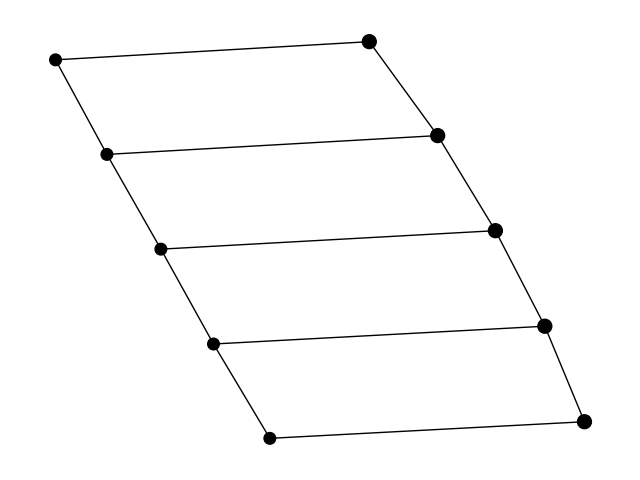
\includegraphics[width=3.0in]{project/fig/ladder10.png}
    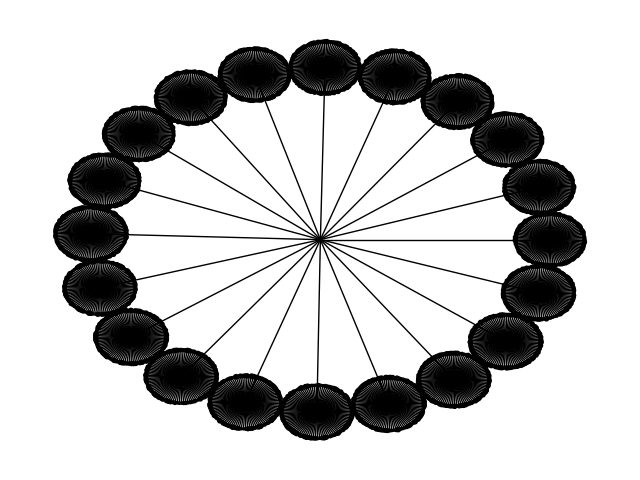
\includegraphics[width=3.0in]{project/fig/star.png}
    \caption{Ladder Graph with 10 Nodes, Star Graph}
    \label{fig:ladder10}
\end{figure}

\subsection{Description of Tree Algorithms and Test Cases}

The final strategies we tested for parallelism within trees are as follows:
\begin{itemize}
    \item Sequential: our sequential algorithm \ref{alg:sequential}
    \item Within Levels: the parallelization strategy described in Section \ref{sec:levels}
    \item Within Levels, Local: the modification to Within Levels described in Section \ref{sec:levels:local}
    \item Within Levels, Reorder: the strategy described in Section \ref{sec:levels} augmented with the technique from Section \ref{sec:reordering}
    \item Within Child: the strategy described in Section \ref{sec:children}
    \item Within Child, Nested: the strategy described in Section \ref{sec:nested} augmenting that of Section \ref{sec:children}
    \item Within Child, Reorder: the strategy described in Section \ref{sec:children} augmented with the technique from Section \ref{sec:reordering}
\end{itemize}

The test inputs are as follows:
\begin{itemize}
    \item Random 1: a random tree on 2000 nodes with 20 parts and cost bounds [400, 600]
    \item Random 2: a random tree on 2000 nodes with 20 parts and cost bounds [400, 600]
    \item Random 3: a random tree on 2000 nodes with 20 parts and cost bounds [300, 600]
    \item Ladder 1000: a ladder graph on 1000 nodes with 30 parts and cost bounds [200, 400]
    \item Star: a multi-level star graph on 2021 nodes with 20 parts and cost bounds [200, 400]
\end{itemize}

\subsection{Parallelism within Tree}

We notice that the parallelism within levels strategy provides no benefit to computation time. 
This is partially because many levels of the tree have comparatively few nodes to parallelize over, as seen in Figure \ref{fig:nodes_per_level}.
In addition, the $O(p)$ critical sections per thread likely cause high contention with the global DP table data structure, so many threads may be stalling when attempting to access this structure.
Updates to this structure may also cause invalidations such that other threads reading this structure for data on different nodes must now re-fetch the data into their caches.

We also notice that the local data structure technique to remove synchronization does not help us fix issues with the parallelism within levels.
As mentioned in Section \ref{sec:levels:local}, this is likely due to the combination of increasing contention by having critical sections at the same time for every thread and having less local memory accesses due to alternating between global and thread-local data structures.

We notice that within-child parallelism is very effective.
The $p$ fixed amounts of work per level are efficiently parallelized over with low amounts of threads.
There is some degree of falloff in efficiency once threads are assigned fewer and fewer pieces of work per thread.
This is also in part due to the asymmetry in number of pieces of work per thread: when some threads have only 3 pieces of work and some 2, the difference in runtime per thread can cause a long period of idleness for some threads.

We also notice that nesting parallelism in the computations of S1 and S2 is not effective.
This is likely due to the extreme amount of contention for the lock needed to update the shared hash map.
That this is an issue with even only 2 threads, one for S1 and one for S2, suggests that this is not a reasonable mode of parallelization (it is fine-grained enough that the benefits from evenly distributing small pieces of work are outweighed by the overhead of managing parallelism).

Finally, we notice that reordering the graph does not significantly change performance.
This is likely because in the vast majority of cases, we are working with relatively low-degree trees.
As such, the entire graph data structure is small (e.g. 16 KB or less for weights and adjacency lists) and large amounts of it can be loaded into the cache and reused in later iterations of the algorithm.
Thus, locality does not provide a significant benefit because we are already not evicting data before we can reuse it later.

\begin{table}[]
    \centering
\begin{tabular}{|l|l|l|l|l|l|}
\hline
          & Random 1 & Random 2 & Random 3 & Ladder 1000 & Star \\ \hline
Sequential & 4.548 & 3.058 & 11.300 & 11.976 & 9.165 \\ \hline
Within Levels (2 threads) & 5.544 & 3.884 & 13.739 & 11.149 & 10.435 \\
Within Levels (4 threads) & 5.482 & 3.807 & 13.545 & 11.601 & 10.688 \\
Within Levels (8 threads) & 5.418 & 3.867 & 13.359 & 12.031 & 10.734 \\ \hline
Within Levels, Local (2 threads) & 5.708 & 3.965 & 14.031 & 11.397 & 11.225 \\
Within Levels, Local (4 threads) & 5.688 & 3.997 & 14.089 & 12.513 & 11.412 \\
Within Levels, Local (8 threads) & 5.649 & 3.951 & 14.059 & 11.748 & 11.546 \\ \hline
Within Levels, Reorder (2 threads) & 5.577 & 3.874 & 13.748 & 11.921 & 10.546 \\
Within Levels, Reorder (4 threads) & 5.491 & 3.814 & 13.453 & 11.876 & 10.726 \\
Within Levels, Reorder (8 threads) & 5.436 & 3.919 & 13.374 & 12.100 & 10.793 \\ \hline
Within Child (2 threads) & 4.864 & 3.357 & 11.842 & 11.839 & 9.534 \\
Within Child (4 threads) & 2.926 & 1.896 & 7.344 & 6.644 & 5.977 \\
Within Child (8 threads) & 1.633 & 1.086 & 4.303 & 3.970 & 4.918 \\ \hline
Within Child, Nested (2 threads) & 3.284 & 2.240 & 7.880 & 8.144 & 7.170 \\ 
Within Child, Nested (4 threads) & 5.950 & 5.188 & 9.153 & 5.360 & 9.081 \\ 
Within Child, Nested (8 threads) & 11.769 & 11.018 & 14.139 & 6.581 & 15.278 \\ \hline
Within Child, Reorder (2 threads) & 4.888 & 3.383 & 11.890 & 11.876 & 9.500 \\
Within Child, Reorder (4 threads) & 2.934 & 1.893 & 7.351 & 6.636 & 5.980 \\
Within Child, Reorder (8 threads) & 1.636 & 1.086 & 4.333 & 4.025 & 4.913 \\ \hline
\end{tabular}
    \caption{GHC Timings}
    \label{tab:ghc-time}
\end{table}


\begin{figure}
    \centering
    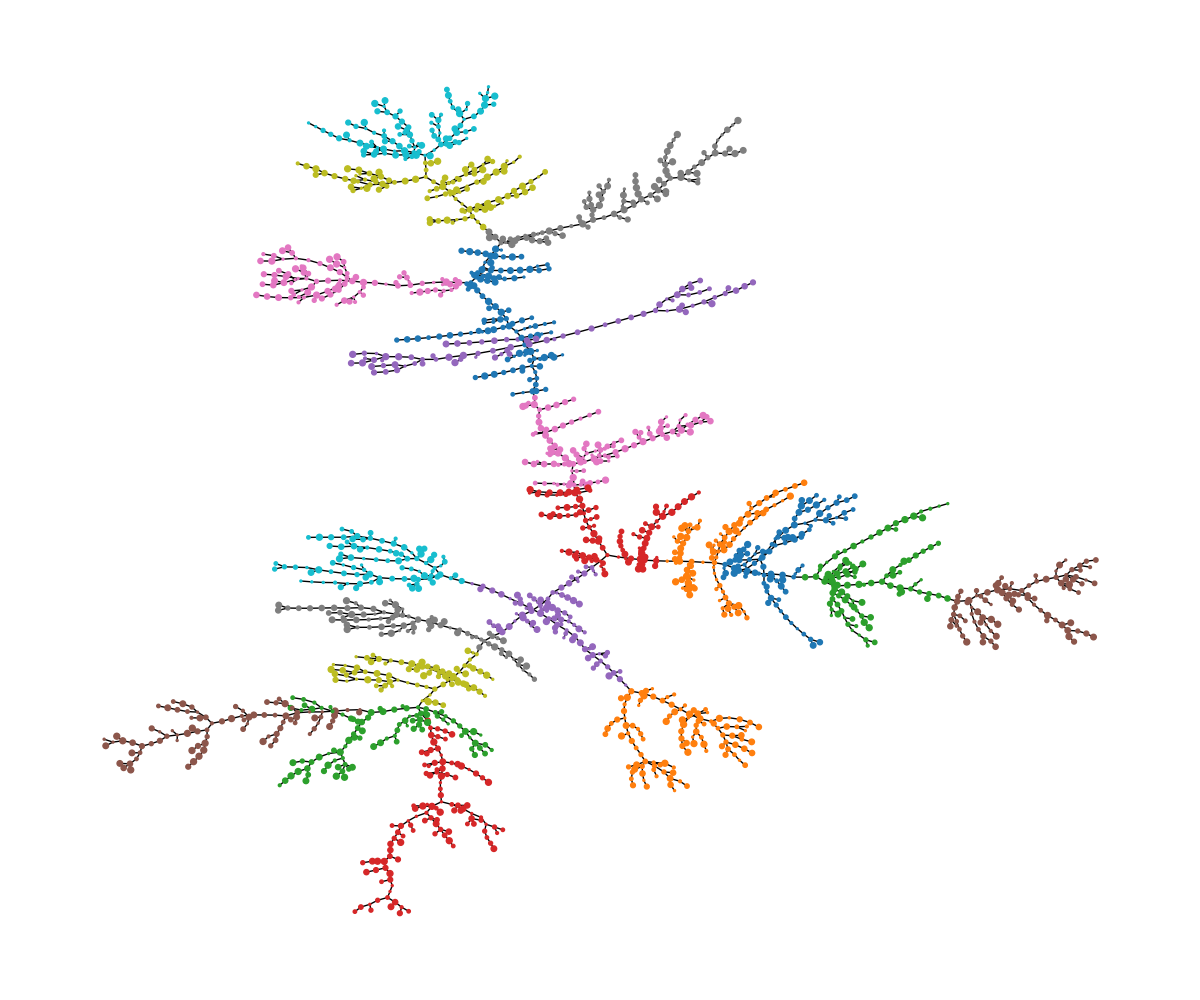
\includegraphics[width=3.0in]{project/fig/assignment_large1_seq.png}
    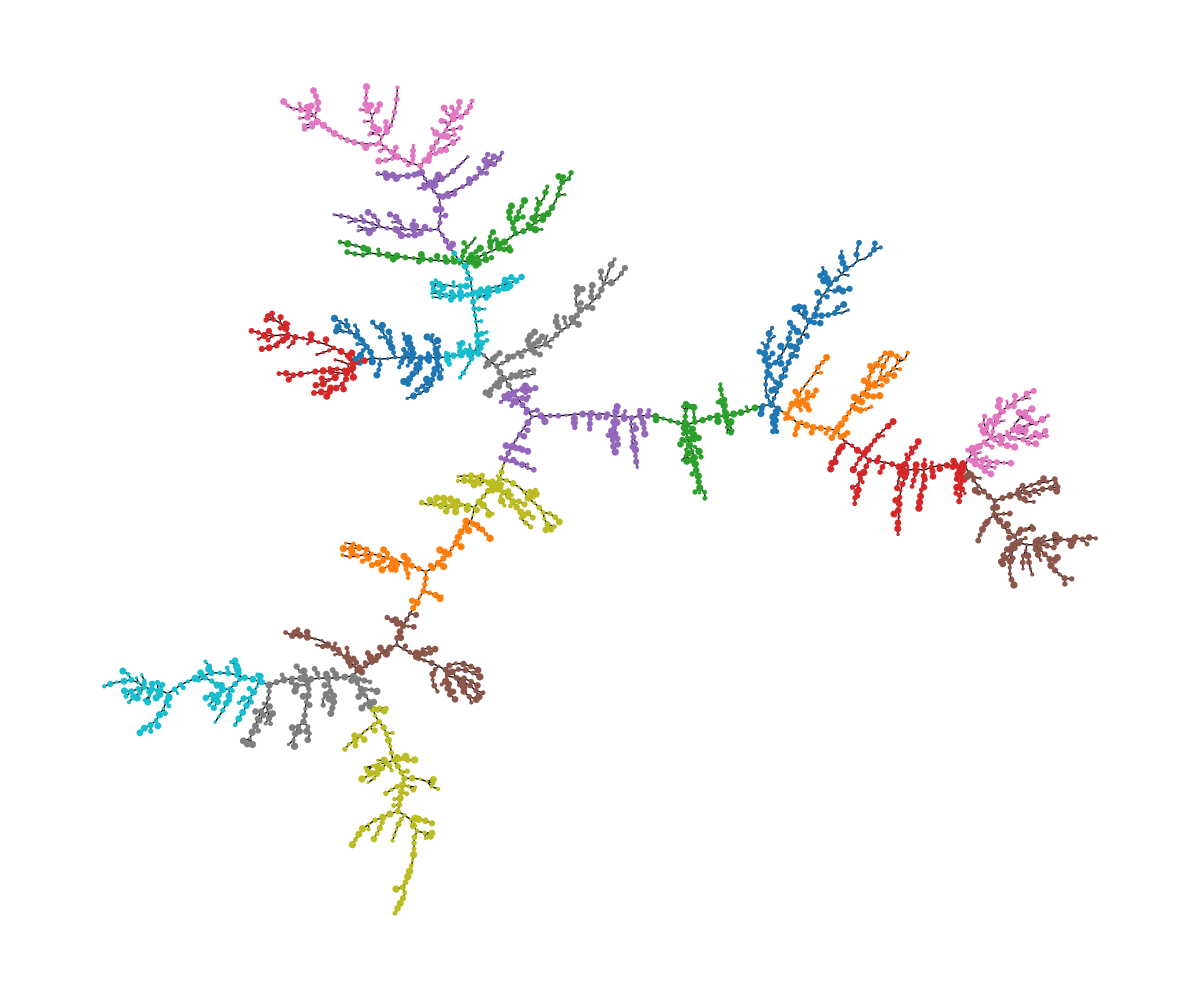
\includegraphics[width=3.0in]{project/fig/assignment_large2_seq.png}
    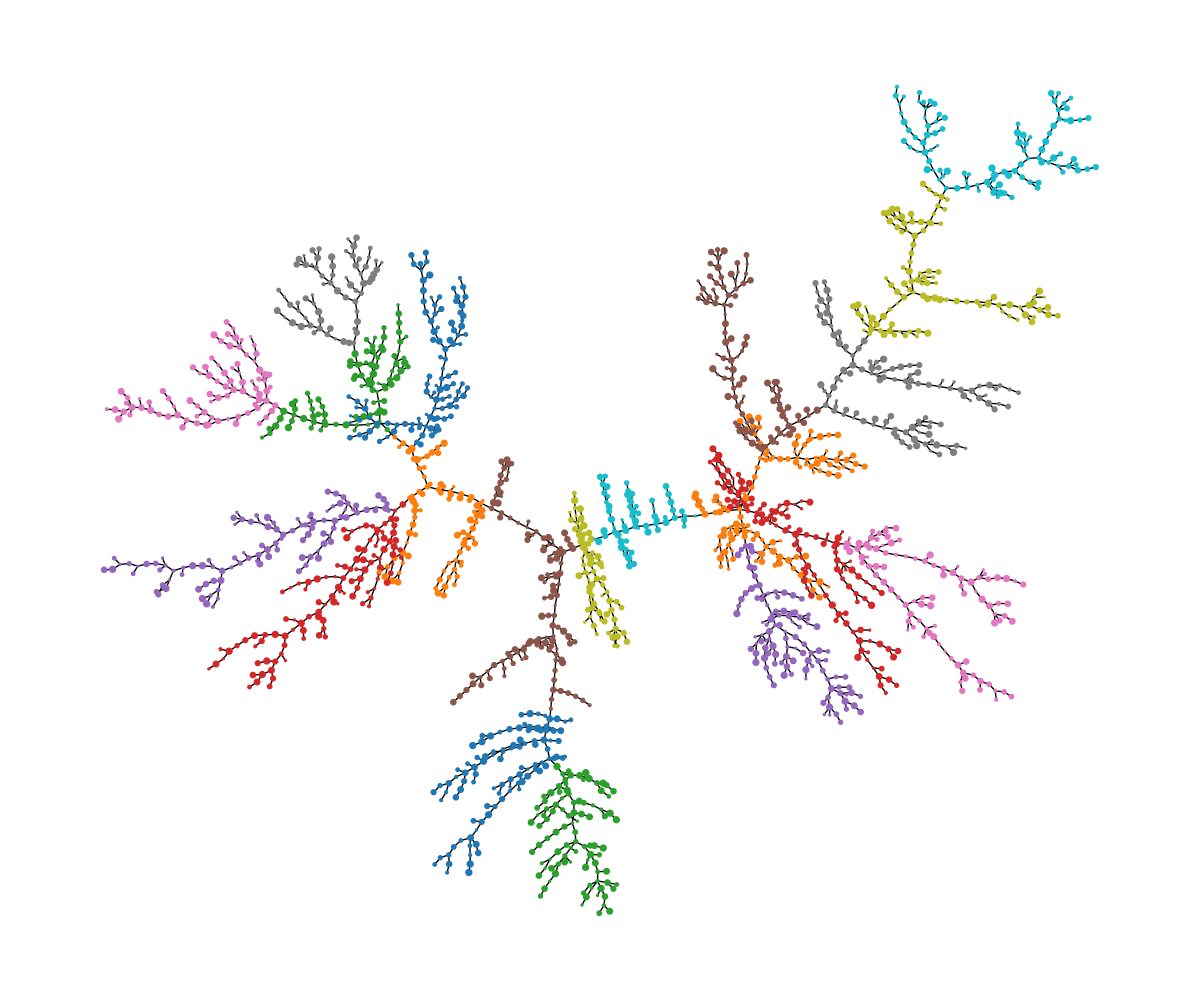
\includegraphics[width=3.0in]{project/fig/assignment_large3_seq.png}
    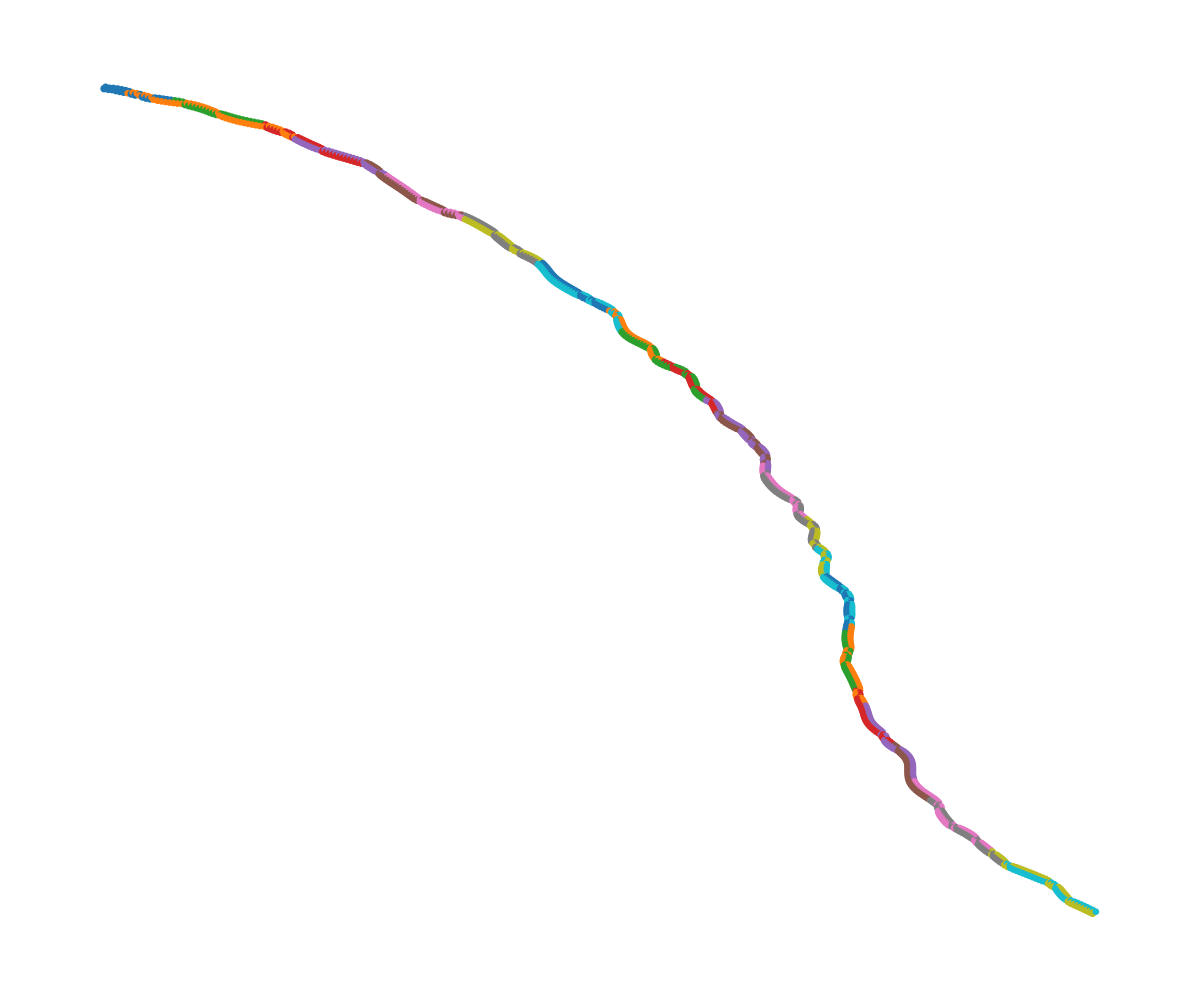
\includegraphics[width=3.0in]{project/fig/assignment_ladder1000_seq.png}
    \caption{Testing Suite Partition Assignments (first row: random tree 1, random tree 2; second row: random tree 3, ladder 1000)}
    \label{fig:assignment}
\end{figure}

\begin{figure}
    \centering
    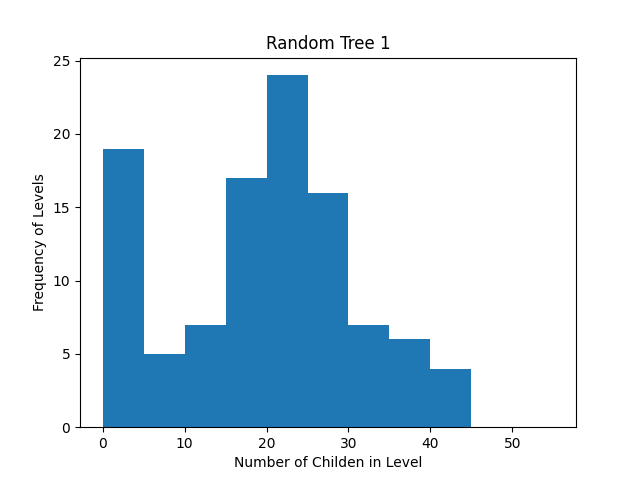
\includegraphics[width=2.0in]{project/fig/large1_postorderlevel.png}
    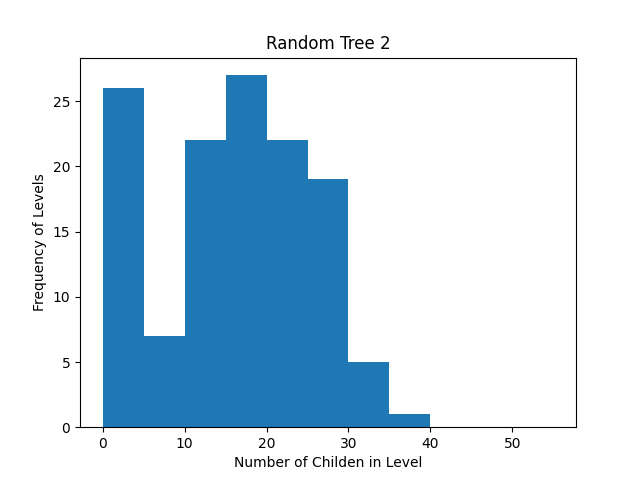
\includegraphics[width=2.0in]{project/fig/large2_postorderlevel.png}
    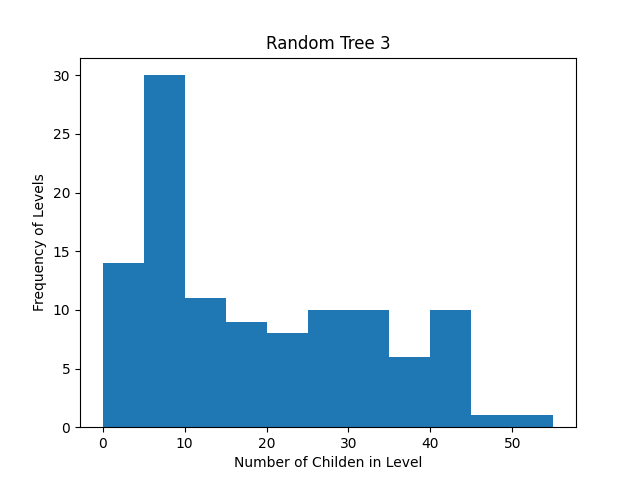
\includegraphics[width=2.0in]{project/fig/large3_postorderlevel.png}
    \caption{Nodes per Postorder Level}
    \label{fig:nodes_per_level}
\end{figure}

\subsection{Parallelism over Spanning Trees}

As noted in Section \ref{sec:trees}, this strategy is effective on harder tasks where multiple spanning trees need to be tried in order to find a valid partition.
We first tested the method of parallelism within a child vs the method of parallelism across trees on both GHC (8 threads) and PSC (32 threads) on the ladder 500 test case with $p = 50, l=77, u=93$ and 40 max iterations, with results shown in Figures \ref{fig:ghc_multiple_tree} and \ref{fig:psc_multiple_tree}.
We then tested the methods on PSC (32 threads) on the ladder 500 test case with $p = 25, l = 165, u = 175$ and 400 max iterations, a test case which has a much lower probability of success for any given spanning tree, with results shown in Figure \ref{fig:psc_multiple_tree_alt}.

We note that the parallelism within a child shows a geometric distribution over runtimes, as expected of the overall runtime of a sequence of random trials with a fixed probability of success.
This corresponds to how we try only a single tree at a time and make this computation as efficient as possible.
The parallelism over trees starts at a much higher baseline number of trees, because each thread starts at least one tree during a run of the algorithm.
However, it is much more effective in terms of runtime per tree, as each tree being tested can be thought of as an optimized sequential implementation of the algorithm, where there is no falloff in efficiency at all from higher numbers of threads.
It thus provides an overall better expected speedup than the sequential algorithm on test cases with a low probability of success.

\begin{figure}
    \centering
    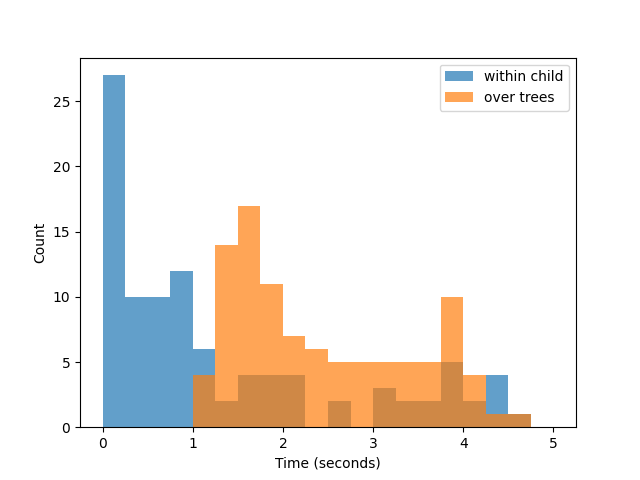
\includegraphics[width=3.0in]{project/fig/ghc_hist.png}
    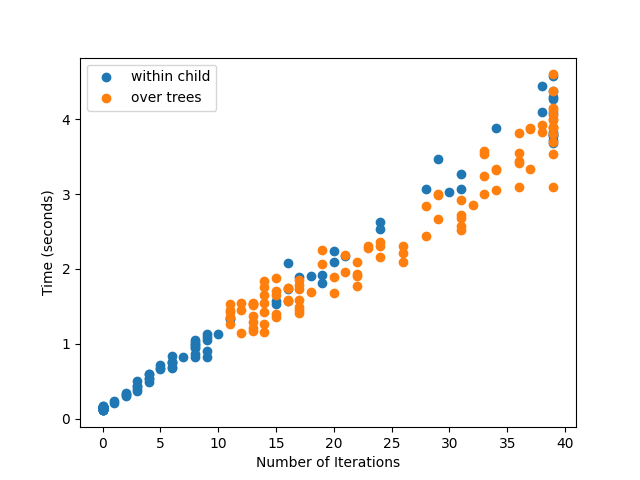
\includegraphics[width=3.0in]{project/fig/ghc_scatter.png}
    \caption{Parallelism within vs across Trees, GHC (8 threads)}
    \label{fig:ghc_multiple_tree}
\end{figure}

\begin{figure}
    \centering
    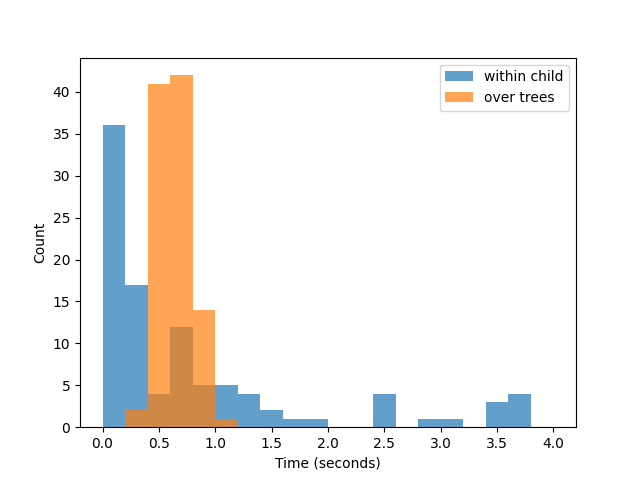
\includegraphics[width=3.0in]{project/fig/psc_hist.png}
    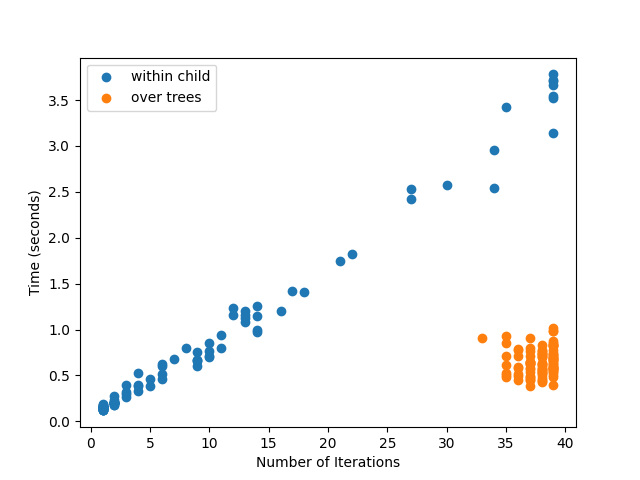
\includegraphics[width=3.0in]{project/fig/psc_scatter.png}
    \caption{Parallelism within vs across Trees, PSC (32 threads)}
    \label{fig:psc_multiple_tree}
\end{figure}

\begin{figure}
    \centering
    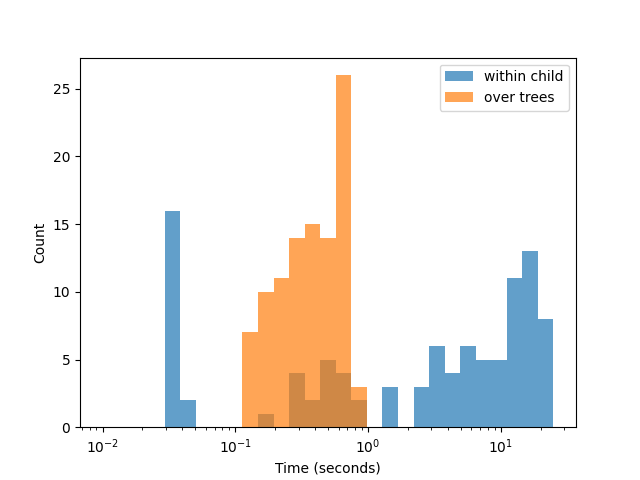
\includegraphics[width=3.0in]{project/fig/psc_alt_hist.png}
    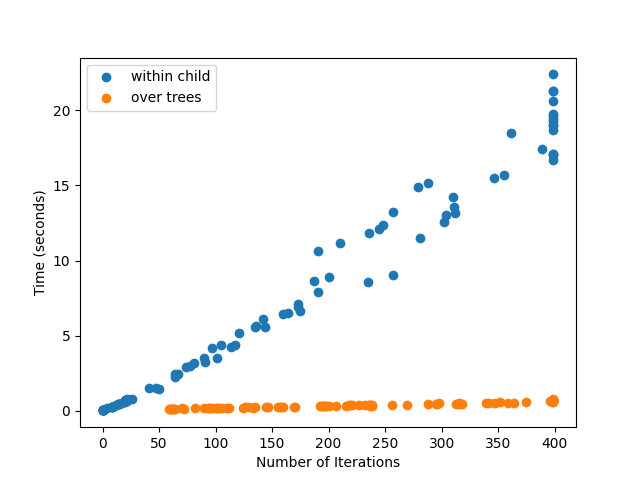
\includegraphics[width=3.0in]{project/fig/psc_alt_scatter.png}
    \caption{Parallelism within vs across Trees, Low Probability Test Case, PSC (32 threads)}
    \label{fig:psc_multiple_tree_alt}
\end{figure}

\subsection{Commentary on Problem Size}

There are 3 variables we may discuss when considering problem size for this task: $p$, the size of the partition to create; $d = u - l$, the range of possible values for the weight of each component; and $n$, the number of nodes in a graph being partitioned.
The runtime of the given algorithm for a single tree is $O(p^4 d^2 n)$.

Differences in the value $p$ can cause drastic increases in runtime for all algorithms.
However, they affect different parallelization strategies in different ways.
Notably, the number of units of work in each batch of parallel work using the parallelism within a child strategy is exactly $p$.
Values of $p$ below the number of processors thus waste execution resources.
We tested both having the number of processors be above and below $p$.

Differences in the value of $d$ may affect runtime, but they do not significantly affect our parallelization strategies.
All parallelization methods must deal with the increased amount of work from having more possible valid partitions.

Differences in the value of $n$ may seem like they affect the parallelism across levels strategy, for which batches of parallel work are batches of nodes.
However, on closer inspection, it can be seen that what matters is not the number of nodes in the overall tree, but the number of nodes in each level, which is primarily determined by the tree topology.
A tree looking similar to a line or ladder graph will never have a large amount of nodes per level, while a tree looking like a star graph will always have at least one relatively large level.
Our testing of different topologies took this behavior into account to provide a more comprehensive evaluation of this parallelization strategy.

\subsection{Commentary on Parallel Device}

We maintain that the multicore CPU is the best choice of common parallel hardware for this task.
The task features a large amount of divergent execution, in which a GPU would not be able to effectively execute tasks in parallel.
The task also features diminishing returns with respect to number of parallel execution contexts at a relatively small number of contexts, so the large number of cores on the GPU may not be able to provide a performance gain simply by not having assignable work.

\bibliographystyle{plain}
\bibliography{references}

\subsection{Codebases}

https://github.com/inkyubeytor/15418-project

https://github.com/inkyubeytor/lupartition

\section*{Work Breakdown}

Work was split 50\%/50\% between partners.

Abhishek Vijayakumar
\begin{itemize}
    \item Implemented graph library.
    \item Implemented sequential algorithm in C++.
    \item Implemented parallelism across levels, both versions.
    \item Implemented nested parallelism within a child.
\end{itemize}

Anna Cai
\begin{itemize}
    \item Implemented test harness.
    \item Created test cases.
    \item Implemented parallelism within a child.
    \item Implemented parallelism over multiple trees.
    \item Implemented visualization system.
    \item Benchmarked all systems.
\end{itemize}

\end{document}
